\newpage

\section{Mockup e navigazione delle finestre}

Il flusso di navigazione all'interno di Symposium è progettato per essere intuitivo e user-friendly. Gli utenti avranno accesso a diverse finestre e schermate chiave per svolgere le loro attività. Ecco un riepilogo del flusso principale:
\begin{enumerate}
	\item \textbf{Schermata principale:} una volta effettuato l'accesso (Figura \ref{login}), gli utenti verranno accolti dalla schermata principale che fornirà una menù generale dal quale gli utenti potranno accedere rapidamente alle funzionalità principali.
	\item \textbf{Creazione di una nuova conferenza:} l'utente sarà in grado di inserire il nome della conferenza, la data, l'orario e la sede. Andando avanti nella fase di creazione l'utente potrà inserire tutti i dettagli delle varie sessioni e accedere infine ad una schermata di riepilogo. (Figura \ref{create})
	\item \textbf{Gestione delle conferenze}
	\item \textbf{Visualizzazione delle conferenze esistenti}
	\item \textbf{Visualizzazione delle statistiche}
\end{enumerate}

\begin{figure}[h!]
	\centering
	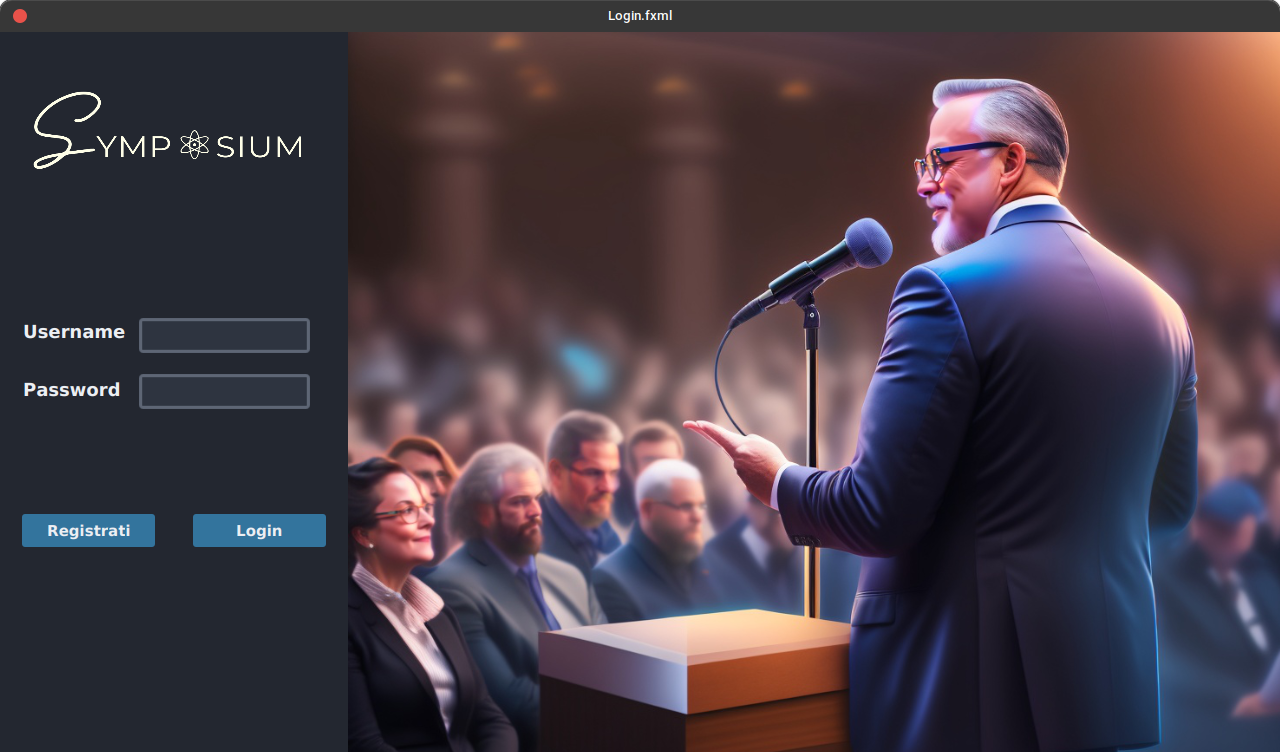
\includegraphics[scale=0.2]{Immagini/Login.png}
	\caption{Schermata iniziale di login}\label{login}
\end{figure}
\begin{figure}[h!]
	\centering
	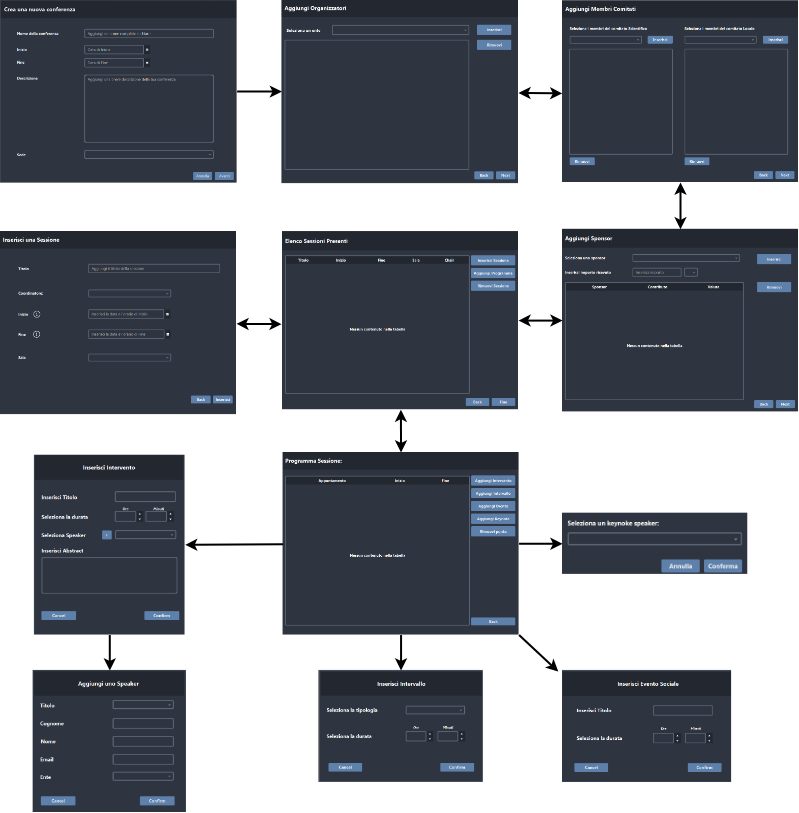
\includegraphics[scale=0.57]{Immagini/Mockup/Create/Flow_Create.png}
	\caption{Mockup delle finestre in fase di creazione}\label{create}
\end{figure}

\begin{figure}[h!]
	\centering
	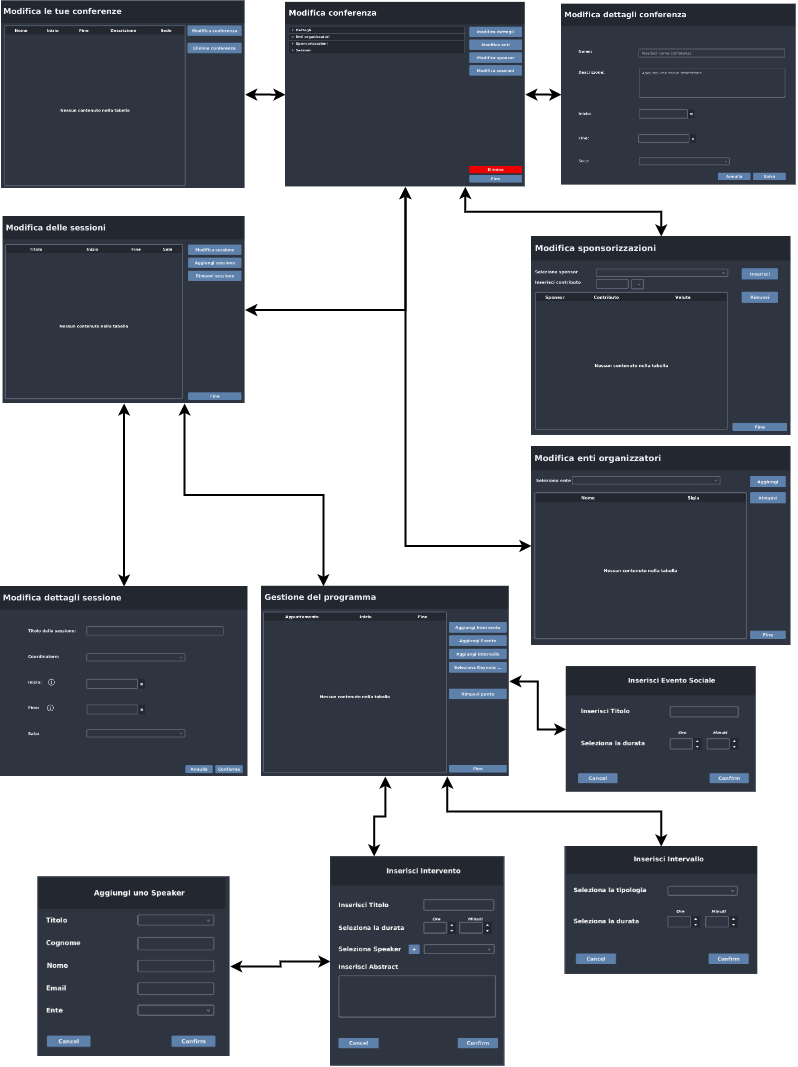
\includegraphics[scale=0.57]{Immagini/Mockup/Edit/Flow_Edit.png}
	\caption{Mockup delle finestre in fase di modifica}
\end{figure}

\begin{figure}[h!]
	\centering
	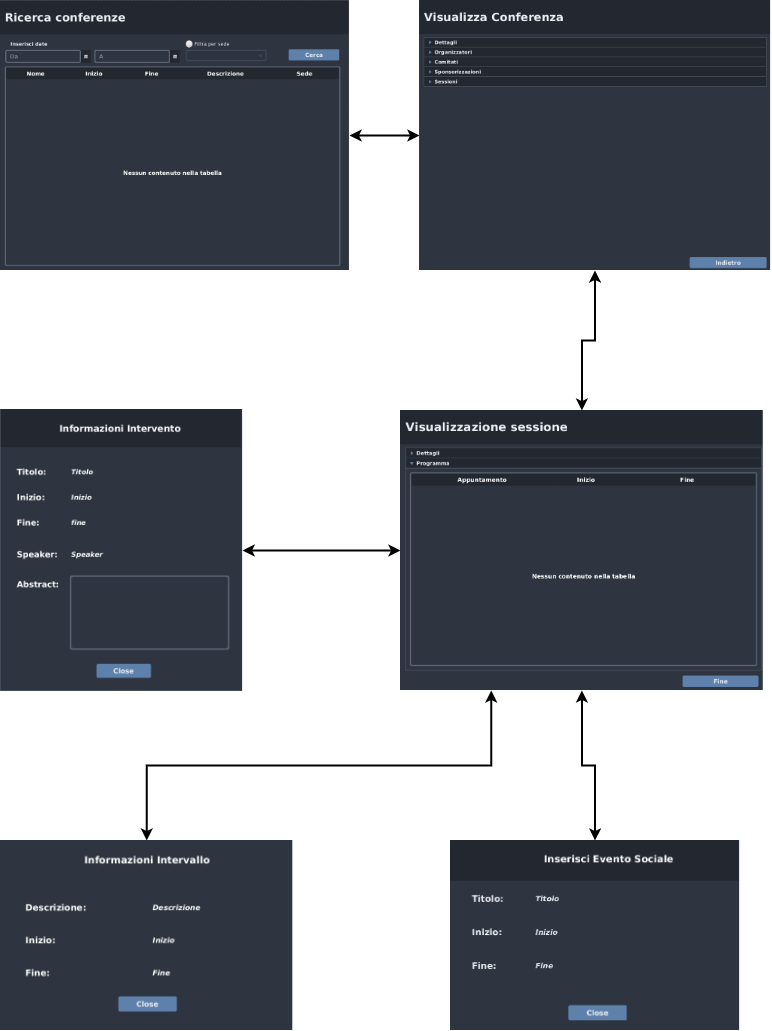
\includegraphics[scale=0.5]{Immagini/Mockup/View/Visualizza_Flow.png}
	\caption{Mockup delle finestre in fase di visualizzazione}
\end{figure}

\begin{figure}[h!]
	\centering
	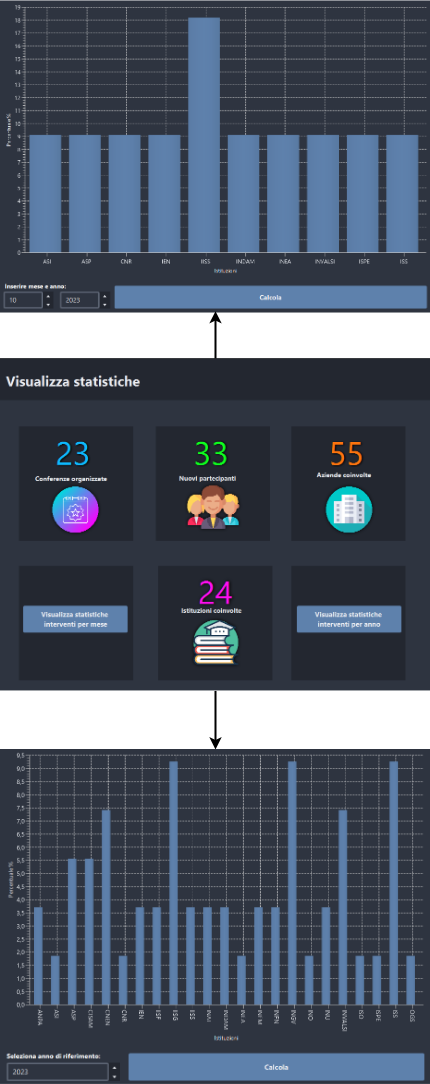
\includegraphics[scale=0.5]{Immagini/Mockup/Stats/Flow_Stats.png}
	\caption{Mockup delle finestre di statistica}
\end{figure}

